\documentclass{article}

\usepackage{NeededPackages}

\title{ATmega328P I/O Ports}
\author{Narendiran S}
\date{\today}

\begin{document}
\maketitle

\section{Introduction}
\begin{itemize}
    \item The directin/drive value/pull-up register of one port pin can be changed without changing the directin/drive value/pull-up register  of any other pin - true \emph{read-modify-write}.
    \item Each output buffer has symmetrical drive characteristics with both high sink and source capability.
    \item All I/Opins have protection diode to both $V_{CC}$ and Ground.
    \begin{figure}[H]
        \begin{center}
            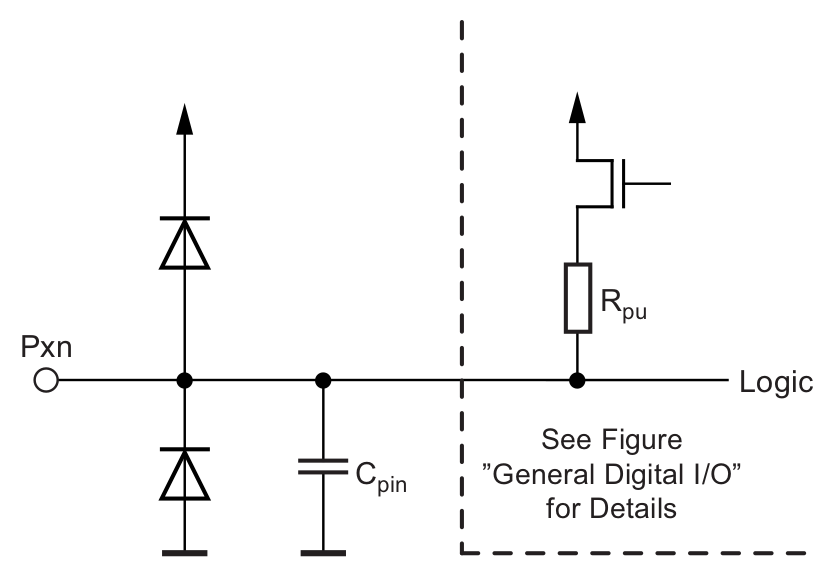
\includegraphics[width=0.5\textwidth]{IOpinEquivalent.png}
        \end{center}
    \end{figure}
    \item Three I/O memory address locations are allocated for each port, one each for the data register – \regFormat{PORTx}, data direction register – \regFormat{DDRx}, and the port input pins – \regFormat{PINx}.
    \item Most pins are multiplexed with alternative functions.
    \item Generally, after reset, the port pins are tri-stated.
    \item Disbaling the \bitFormat{PUD} bit in \regFormat{MCUCR} register disables the pull-up function of all pins.
    \item Unconnected pins should not float and must be connected to internal pull-up or external pull-up/pull-down registor.
\end{itemize}


\section{General Digital I/O}
\begin{figure}[H]
    \begin{center}
        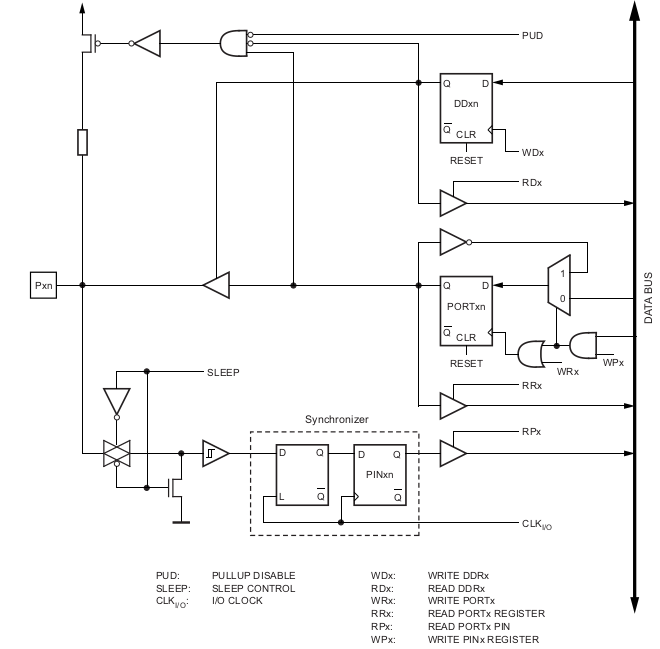
\includegraphics[width=1\textwidth]{IOcomplete.png}
    \end{center}
\end{figure}

\subsection{DDR Registers}
\begin{itemize}
    \item It is used to select the direction of a pin.
    \item DDxn == 1 $-->$ Pin n of Port x is configured as output.
    \item DDxn == 0 $-->$ Pin n of Port x is configured as input.
\end{itemize}

\subsection{PORT registers}
\begin{itemize}
    \item If the pin is configured as Output - Drive the pin.
    \begin{itemize}
        \item PORTxn == 1 $-->$ Pin n of Port x is driven to logic HIGH.
        \item PORTxn == 0 $-->$ Pin n of Port x is driven to logic LOW.
    \end{itemize}
    \item If the pin is configured as Input - configure pull-up resistor.
    \begin{itemize}
        \item PORTxn == 1 $-->$ Pin n of Port x has pull-up resistor activaed.
        \item PORTxn == 0 $-->$ Pin n of Port x has pull-up resistor deactivaed.
    \end{itemize}
\end{itemize}

\subsection{PIN Registers}
\begin{itemize}
    \item It is used to read the status of a pin.
    \item Writing 1 to a PINxn makes the Pin n of Port x toggle.
\end{itemize}

\section{Alternate Port Functions}
\begin{figure}[H]
    \begin{center}
        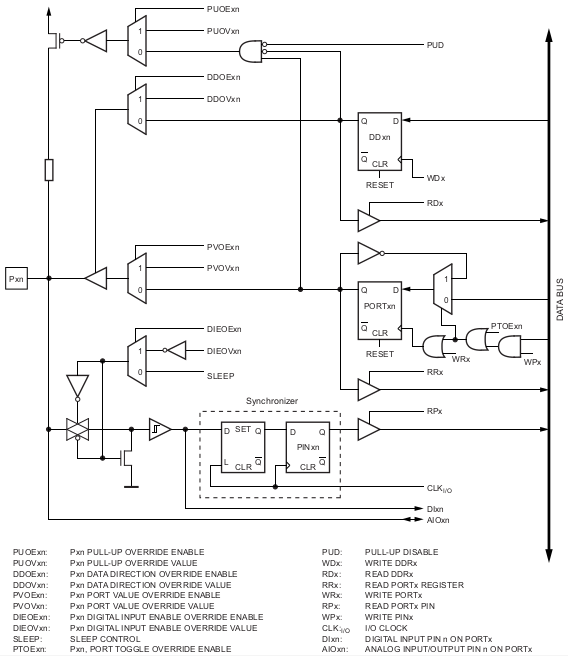
\includegraphics[width=1\textwidth]{IOalternatefunc.png}
    \end{center}
\end{figure}

\begin{figure}[H]
    \begin{center}
        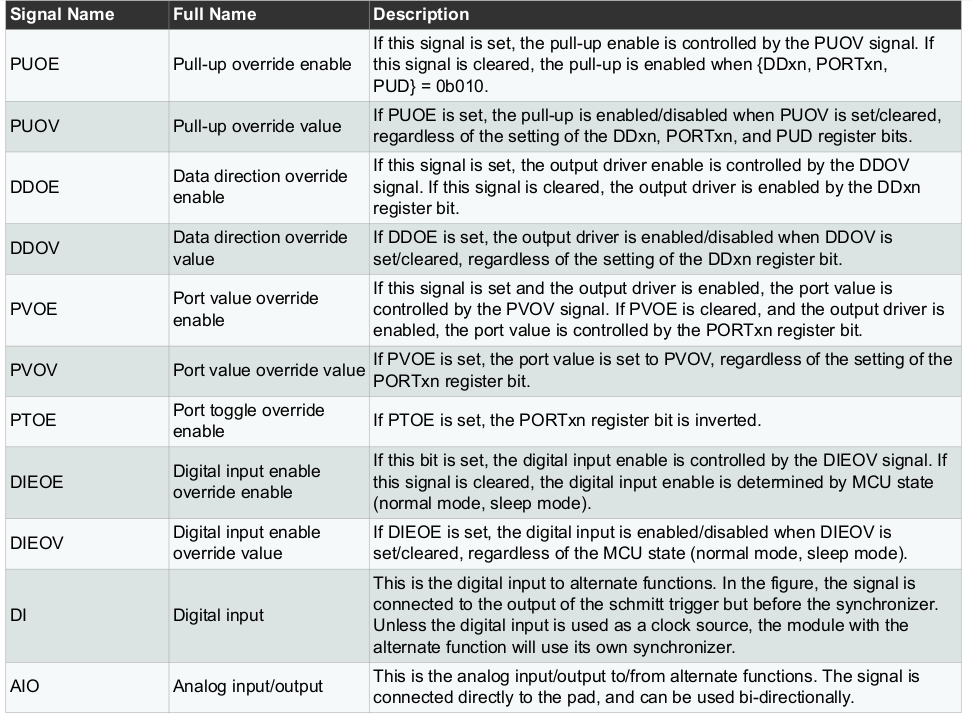
\includegraphics[width=1\textwidth]{IOsignals.png}
    \end{center}
\end{figure}


\end{document}

